\documentclass[12pt]{article}
% This first part of the file is called the PREAMBLE. It includes
% customizations and command definitions. The preamble is everything
% between \documentclass and \begin{document}.

\usepackage[margin=1in]{geometry}  % set the margins to 1in on all sides
\usepackage{graphicx}              % to include figures
\usepackage{amsmath}               % great math stuff
\usepackage{amsfonts}              % for blackboard bold, etc
\usepackage{amsthm}                % better theorem environments

\usepackage{rotating} % for sideway table
\usepackage{xcolor}
\usepackage{hyperref}
\hypersetup{
    colorlinks,
    linkcolor={red!50!black},
    citecolor={blue!50!black},
    urlcolor={blue!80!black}
}

% various theorems, numbered by section

\newtheorem{thm}{Theorem}[section]
\newtheorem{lem}[thm]{Lemma}
\newtheorem{prop}[thm]{Proposition}
\newtheorem{cor}[thm]{Corollary}
\newtheorem{conj}[thm]{Conjecture}

\DeclareMathOperator{\id}{id}

\newcommand{\bd}[1]{\mathbf{#1}}  % for bolding symbols
\newcommand{\RR}{\mathbb{R}}      % for Real numbers
\newcommand{\ZZ}{\mathbb{Z}}      % for Integers
\newcommand{\col}[1]{\left[\begin{matrix} #1 \end{matrix} \right]}
\newcommand{\comb}[2]{\binom{#1^2 + #2^2}{#1+#2}}

\usepackage{array,tabularx}

\newenvironment{conditions*}
  {\par\vspace{\abovedisplayskip}\noindent
   \tabularx{\columnwidth}{>{$}l<{$} @{${}={}$} >{\raggedright\arraybackslash}X}}
  {\endtabularx\par\vspace{\belowdisplayskip}}

\title{Prelim paper}
\author{Anh Le}


\begin{document}
\maketitle

\section{Introduction}
\label{sec:introduction}

Once disregarded as mere ``window-dressing,'' authoritarian institutions have garnered the attention of scholars as an important tool for power sharing, which, in turn, leads to various substantive effects, including regime survival, increased investment, and better economic performance \citep{Gandhi2008}.

While our understanding of authoritarian institution has branched to numerous substantive topics, its causal root deserves more careful studies. Given its common definition as the ``rule of the game'', institutions are fundamentally a set of constraints on human interactions, and thus its effect must be most evident in the interaction between strategic actors itself.  When scholars study the effect of institutions on various substantive areas, inevitably the causal chain must pass through the strategic actions of the actors, mainly with the logic of credible and regular spoil sharing (Svolik, Przeworski). This causal step is theoretically crucial to all of our findings regarding authoritarian institutions. The goal of this article is, therefore, to empirically examine it.

Beyond its theoretical contribution, a study of violence in partially liberalized dictatorship has immense real-world importance. Indeed, violence during periods of political liberalization is the greatest concern of many would-be democrats living under authoritarian regimes. For example, Chinese citizens show overwhelming enthusiasm when asked about democratic features such as popular accountability, separation of power, and political liberalism, yet remain consistently cautious of instability caused by transition (Chu 2008, 309). Therefore, understanding the pattern of violence during liberalization is crucial for the prospect of democracy.

The article will proceed as follows. \Cref{sec:argument} presents an overview of the theoretical argument and empirical analyses. \Cref{sec:theory} posits two theoretical explanations for the effect of legislature on violence. \Cref{sec:empirics_largeN} uses a Bayesian hierarchical model to analyze political violence in authoritarian regimes post-Cold War, showing that the legislature has a modest positive effect. \Cref{sec:empirics_survey} uses a survey experiment to demonstrate that co-optation strategy does prompt Vietnamese business to interact with the regime, a pre-requisite for any material outcome such as violence to change. \Cref{sec:conclusion} concludes.
\section{Theory: Authoritarian legislature and its effect on political violence}

\subsection{Legislature reducing violence}

To consider whether violent means is chosen to reach their goal, we need a theoretical framework to understand how the opposition and the regime engage in the bargaining game. A possible starting point is the bargaining models developed for democratic legislatures, where bargaining outcomes are driven by various institutional rules (positive and negative rule, sequencing of these powers, first-mover advantage, etc.) (Baron and Ferejohn 1989; Cox 2006). However, this type model is not suited to analyze the bargaining under an authoritarian regime, where the institutional rules themselves are under constant threat of being revised by the final arbiter that is violence. In other words, the end game of legislative bargaining now has an extra node that is whether either side will violently suppress the other’s demand. Given this context, the decision of the autocrat and the opposition is better characterized as a bargaining game in anarchy, very much like the bargaining between two sovereign states with the option of going to war (Fearon 1995).

To formally model the interaction, let the negotiation between the opposition and the regime be about the share $x$, $(0 < x < 1)$ of a good (normalized as 1) given to the opposition. (For concreteness we can think of this as the share of the economy’s rent or capital stock). Both sides have the option 1) to bargain and decide on x, or 2) to engage in violent protest / repression. Violence is costly compared to peaceful negotiation---we call this difference in relative cost $c_A$ and $c_O$ for the autocrat and the opposition, respectively. If violence happens, whichever side emerges victorious decides the share x to his heart’s desire---i.e. the winning autocrat would give 0 to the opposition and the winning opposition would give 1 to itself.

Given the uncertain nature of collective action battles, the utility of engaging in violence for the two sides is best formulated as an expected utility that depends on the probability of the opposition winning (call this probability $p$). Thus, the expected utility of the opposition is $p – c_O$, while the expected utility of the ruling regime is $1 - p - c_A$. These two expected utilities sum to less than one, which raises the puzzle why the two sides fail to engage in ex-ante bargaining that splits the difference, giving both sides a higher payoff than the expected utility of violence. Indeed, any amount of x between $(p - c_O, p + c_A)$, i.e. the bargaining range, is more desirable than violence to both sides.

Yet war happens between states and so does violence under authoritarian regimes. The international relations literature suggests three factors that may lead to violence, all of which having a legislature can help alleviate.

\begin{enumerate}
\item Information asymmetry regarding $p$

Due to the incentive to bluff, both sides only have incomplete information about the capability of the other. This leads to differing estimate of $p$, leading to non-overlapping preferences. This information asymmetry can be alleviated by having an elected legislature that helps the autocrat identify the collective action capability of the opposition. During regular legislative sessions, the regime can observe the position of opposition legislators to gauge their unity strength. Furthermore, during elections, both sides’ mobilization effort provides information to the other about its collective action capability without actually resorting to violence. The real, competitive stake of these elections also means that both sides are exerting its best effort, reducing the risk of bluffing and deception. Therefore, the autocrat can trust the information it receives about the opposition’s capability $(p)$, and consequently has a better idea about the political constraint that it faces.

\item The bargaining range $(p - c_O, p + c_A)$ depends on the value of $c_O and c_A$

Having an elected legislature can also increase $c_A$ and $c_O$, i.e. the cost of violence compared to peaceful negotiation. First, elections provide the opposition with a platform to influence policy making without resorting to violence (Rigger 1999, 14). Despite inevitable electoral manipulations, voters still know who the candidates are and can vote in support of their message. While these votes will not dethrone the regime, they serve as an informal referendum that alerts the regime about the popularity of its policies. In this way, the opposition can influence the agenda without winning the election itself. Indeed, if participation in the electoral game proves to be an attractive option to the opposition, radicalizing becomes relatively more costly as a means of gaining influence.

Second, in Dahlian terms, elections also tempt the ruling regime to stay within the institutionalized game by raising the cost of repression (Dahl 1971, 15). Indeed, elections “open up avenues of collective protest” by creating convergent social expectations that are both large in scope (affecting all citizens) and concentrated in time frame (Schedler 2009). Furthermore, by participating in elections, the opposition builds up its organizational strength, which can be used to mobilizing votes as well as organizing protest (Thompson and Kuntz 2004).

In addition, upholding elections and institutional bargaining is an attractive option for regimes to build their legitimacy and assuage grievances about past infractions (Lindberg 2009, 339). By adapting its policies based on election results, the regime can also bring its position closer to the popular will in incremental steps, each with acceptable cost. Indeed, it is not contradictory to say that an authoritarian regime may protect voters’ rights or respond to their demands as a strategy for the regime to stay in power, because there are often hard-liners and reformists within the regime. If the reformists’ strategy of electoral engagement proves to be a successful alternative to maintain power, more members of the regime will be tempted to become liberal-minded.

\item Unit indivisibility: the contested good may not be divided continuously

A final possibility that leads to violence is that the opposition and the ruling regime may be fighting over issues that cannot be continuously divided. For example, were the contested issue about whether religious law should be adopted, it may not be possible to split the issue space to arrive at a compromise within the (p - cO, p + cA) range. An elected legislature again ameliorates this problem. By providing an arena in which both sides can engage in multiple negotiations along many policy issues, it provides more opportunities for side payments. In contrast, were the opposition shut out of the policy making entirely, the only way they could gain influence is to arouse the populace to violent protest. The best way to do so is not via a nuanced discussion of multiple policy points but an intense focus on a highly contentious issue, further exacerbating the problem of unit indivisibility. Therefore, we should expect elected legislature to provide better opportunities for negotiation.

In sum, the overarching of over these causal mechanisms is that the elected legislature provides an arena for the ruling and the opposition to interact, gain information, and adjust strategies. In game theoretic sense, by lengthening the horizon and improve the regularity of stakes, repeated interaction encourage players to think about the future and deter the temptation to radicalize. Overall, these effects encourage incremental changes over radical tactic and favor cooperation over defection (Axelrod 1984). This leads to our hypothesis that:

H1: Authoritarian regimes that create a legislature will experience less violence in its interaction with the dissidents.
\end{enumerate}

\subsection{Legislature increasing violence}
Throughout the previous model, it is implied that the actors’ utility functions remain static with the only parameters being the cost of violence and the share of the issue space. Yet this assumption may miss the dynamism of the opposition’s democratic expectation, which becomes increasingly demanding as the regime starts liberalizing.

Speaking about this issue, Ted Gurr hypothesizes, “The potential for collective violence varies strongly with the intensity and the scope of relative deprivation among members of a collectivity.” Relative deprivation, in turn, is defined as the perceived discrepancy between value expectation (what people believe they are entitled to) and value capability (what the people believe they are able to attain) (1970, 24). Seen under this light, repeated elections may increase the potential for political violence by raising the democratic expectation, which can lead to violent protest if unfulfilled. The effect of elections is especially potent because it affects all citizens, thus raising not only the intensity but also the scope of relative deprivation.

Indeed, unfulfilled political expectation is a common case of relative deprivation causing violence. Historical examples are numerous, spanning various time periods as well as scopes of conflict: from the Puritan Revolution of 1640-60, which was sparked by attempts of the Stuart kings to reinstate royal absolutism, to the protest in twentieth-century colonies, which often followed the imposition of restrictions after a period of political liberalization (1970, 115). This pattern makes sense because, when people have tasted freedom, not only do they want more rights but they also consider rights more important. In other words, the opposition may not simply optimize its share of the issue space but also develops a minimum level of acceptable concession. If opposition’s expectation rises too quickly, the ruling regime may not have enough time to appropriate adjust their position especially if the hard-liners are also trying to retrench given signs of a political spiral. For this reason, it is plausible that electoral authoritarianism leads to more violent interaction between the ruling regime and the opposition.
\section{Empirics}

\subsection{Description of data}

\begin{itemize}

\item Dependent variable: \textit{legislature}, operationalized as $LIEC \geq 5$ 

As my theoretical argument emphasizes the role of the legislature as an informational and commitment device, I code a country-year as having a legislature if multiple parties are legal. Even if opposition parties do not win seat, the electoral process also conveys information about the organizational strength and the preference of both sides. This coding rule operationalizes as having LIEC (Legislative Index of Electoral Competitiveness) be 5 or higher in the DPI (Database of Political Institutions).\footnote{The values LIEC are as follows: 4---1 party, multiple candidates; 5---multiple parties are legal but only one party won seats; 6---multiple parties did win seats but the largest party received more than 75\% of the seats; 7---largest party got less than 75\% (DPI 14)}

\item Independent variable: \textit{violence} in regime-dissident interaction

Using a dataset of machine coded news reports around the world from 1991-2012, I am able to look at individual events that happened between the regime and the dissident, enabling an analysis at a highly granular level. These event data come from ICEWS (Integrated Crisis Early Warning System), a project funded by DARPA (Defense Advanced Research Projects Agency) to aid the US policy makers in predicting and responding to crises around the world . These news articles are harvested from ``over 75 international sources (AP, UPI, and BBC Monitor) as well as regional sources (India Today, Jakarta Post, Pakistan Newswire, and Saigon Times),'' ensuring comprehensive coverage  (cite O'Brien 2010 (94), 2013). While this dataset has been de-duplicated once so that an event covered by multiple news report only shows up once, I created my own filter to delete duplicates that share the same source actor, target actor, and happen at the same time and place.

These text data are then processed with Schrodt's TABARI event data coding system to determine the nature and the intensity of the reported political activity. In addition, the event is matched with a dictionary of actors (with over 8,000 entries) that further divides into five broad categories: religious, governmental, dissidents, business, and other. In sum, from this database I am able to extract any interaction between the government and the dissident, where and when it happens, and its level of violence (measured by the Goldstein score\footnote{The Goldstein score is a measure of intensity of conflict or cooperation, developed by Joshua S. Goldstein. The score has values from -10 (Military attack, clash, assault), 0 (Explain or state policy, state future position) to 8.3(Extend military assistance) See Goldstein 375 for how the event types are coded into this scale).}
\end{itemize}

\subsection{Empirical strategy}

First, my empirical strategy improves over the extant literature with a careful choice of country-years to study. Scholars in the authoritarian legislature have customarily count all authoritarian country-years with an existing legislature in the sample. However, this risks including dictatorships that passively inherited the legislature from the previous regime, who would rather abolish the institution if not for the fear of backlash. On the spreadsheet, such cases would look identical to an autocrat opening up to co-opt the opposition, yet the logic is entirely different. To use a cautionary example, in Preworski and Gandhi (1283), the legally enforced two-party legislature under the Brazilian junta government is not a reformist institution created by the autocrat to facilitate power sharing but a gutted down legislature when the election result did not go the regime's way. To guard against this possibility, I only look at authoritarian regimes that created  legislature during its rule as the ``treatment'' group. (From now on, I will use ``treatment'' as a shorthand for the creation of the legislature).

Second, it is important to recognize that an authoritarian regime without a legislature is not the correct counter factual, and thus make a very poor control group. Indeed, a regime may not create a co-opting legislature because there is never a sufficient threat of violence from the opposition. Therefore, even though we may see that regimes without legislature are very peaceful, this does not mean that a legislature has no effect on regime-dissident interaction. Conversely, a regime under rising violent threat may institute a legislature that successfully puts a lid on the growing discontent. However, since the level of violence is now constant, it will look as though the legislature had no effect.

To setup the correct counter factual, I use matching to create a sample of comparable cases. The crux of the strategy is to find two country years similar along all covariates in year $t$ (including $\text{violence}_t$), but one has a legislature in the next year while the other does not. Then, the difference in violence between these two cases in the ensuing period is attributable to the legislature.

This strategy is implemented as follows. First, to construct the treated population, I look at all country years in which an authoritarian legislature is created and build a four-year panel around it, including the one year before the treatment, and the three years after. Second, to construct the control population, I build similar four-year panels from all the other authoritarian country years without a legislature. Finally, for each panel in my treated population, I find its closest match from the control population based on their first year (which is the pre-treatment year for the treated countries). I match on level of violence and other covariates as reported in \autoref{tab:matching_balance_largen}, significantly improving the balance across the board. The matched pairs of panel are reported in \autoref{tab:matched_pairs}. Given that factors that affect violence may have various non-linear effect, matching alleviates the serious concern about functional misspecification. 

In general, matching alone does not recover the correct causal inference when there is selection based on unobservables. However, in this case, it addresses the most important concerns. First, as discussed above, matching on the level of violence in the pre-treatment year creates a sample of regimes with similar violence trajectory, and thus sets up the correct counter factual. Second, even though there is a risk of regimes creating legislature in anticipation of violence, this requires a significant ability from the regime to monitor the capability and the preference of the opposition. In the absence of a legislature, this information is likely to come from the security apparatus---therefore, the military expenditure (as a percentage of GDP) is matched on as a proxy control for the regime's capacity to anticipate violence.

\begin{sidewaystable}[ht]
\centering
\begin{tabular}{lrrlrrrl}
  \hline
 & \multicolumn{2}{c}{Pre-Match} &   \multicolumn{2}{c}{Post-Match} \\
Covariate & Treated mean & Control mean & p-value & Treated mean & Control mean & p-value &  \\ 
  \hline
Ethnic Fractionalization \_ & 0.61 & 0.59 & 0.59 & 0.61 & 0.60 & 0.81 &  \\ 
Violence (Goldstein score) & -4.50 & -4.05 & 0.51 & -4.50 & -4.49 & 0.94 &  \\ 
$\text{Violence}^2$ & 29.84 & 23.22 & 0.34 & 29.84 & 29.03 & 0.65 &  \\ 
Regime duration (years) & 12.08 & 34.30 & 0.00*** & 12.08 & 12.71 & 0.71 &  \\ 
$\text{Regime duration}^2$ & 278.00 & 2783.57 & 0.00** & 278.00 & 287.38 & 0.89 &  \\ 
Military & 0.08 & 0.06 & 0.67 & 0.08 & 0.12 & 0.57 &  \\ 
Monarchy & 0.04 & 0.25 & 0.00*** & 0.04 & 0.04 & 1.00 &  \\ 
Party & 0.29 & 0.48 & 0.07* & 0.29 & 0.29 & 1.00 &  \\ 
log(gdp) & 22.65 & 23.95 & 0.00*** & 22.65 & 22.78 & 0.67 &  \\ 
log(gdp per capita) & 7.63 & 8.58 & 0.00*** & 7.63 & 7.65 & 0.95 &  \\ 
Military expenditure (\% of GDP) & 2.44 & 4.34 & 0.00*** & 2.44 & 2.40 & 0.89 &  \\
Land (1000 $\text{km}^2$)& 760.22 & 1674.68 & 0.00*** & 760.21 & 783.37 & 0.80 &  \\ 
Population (million) & 22.62 & 140.73 & 0.00*** & 22.62 & 21.74 & 0.90 &  \\
Natural Resource Export (\% of GDP) & 14.79 & 22.64 & 0.03** & 14.79 & 14.16 & 0.72 &  \\ 
Resource $\times$ Ethnic & 8.61 & 14.43 & 0.01** & 8.61 & 8.33 & 0.82 &  \\ 
   \hline
\end{tabular}
\caption{Pre and Post-Matching Balance}
\label{tab:matching_balance_largen}
\end{sidewaystable}

\begin{table}[ht]
\centering
\begin{tabular}{lrlr}
  \hline
 \multicolumn{2}{c}{Treatment} &   \multicolumn{2}{c}{Control} \\
Country & Year & Country & Year \\ 
  \hline
Algeria & 1996 & Sudan & 1992 \\ 
  Angola & 1992 & Angola & 2000 \\ 
  Azerbaijan & 1992 & Uganda & 1991 \\ 
  Belarus & 2004 & Belarus & 2000 \\ 
  Cambodia & 1993 & Laos & 1999 \\ 
  Central African Republic & 2005 & Uganda & 2001 \\ 
  Chad & 1997 & Central African Republic & 1992 \\ 
  Congo, Republic & 2002 & Nigeria & 1994 \\ 
  Congo, Dem Rep & 2006 & Congo, Dem Rep & 1996 \\ 
  Ethiopia & 1995 & Ethiopia & 1993 \\ 
  Gambia & 1996 & Belarus & 2001 \\ 
  Ghana & 1995 & Belarus & 2000 \\ 
  Jordan & 1993 & Swaziland & 2007 \\ 
  Kazakhstan & 1995 & Sudan & 1994 \\ 
  Kenya & 1992 & Laos & 1997 \\ 
  Kyrgyzstan & 1995 & Belarus & 1998 \\ 
  Pakistan & 2002 & Algeria & 1993 \\ 
  Rwanda & 2003 & Rwanda & 1999 \\ 
  Sudan & 2000 & Sudan & 2006 \\ 
  Tajikistan & 1995 & Belarus & 1999 \\ 
  Tanzania & 1995 & Sierra Leone & 1992 \\ 
  Togo & 1994 & Togo & 1991 \\ 
  Uganda & 2006 & Uganda & 1998 \\ 
  Uzbekistan & 1999 & Ethiopia & 1993 \\ 
   \hline
\end{tabular}
\caption{The matched sample of country years}
\label{tab:matched_pairs}
\end{table}
\documentclass[12pt]{article}

% This first part of the file is called the PREAMBLE. It includes
% customizations and command definitions. The preamble is everything
% between \documentclass and \begin{document}.

\usepackage[margin=1in]{geometry}  % set the margins to 1in on all sides
\usepackage{graphicx}              % to include figures
\usepackage{amsmath}               % great math stuff
\usepackage{amsfonts}              % for blackboard bold, etc
\usepackage{amsthm}                % better theorem environments


% various theorems, numbered by section

\newtheorem{thm}{Theorem}[section]
\newtheorem{lem}[thm]{Lemma}
\newtheorem{prop}[thm]{Proposition}
\newtheorem{cor}[thm]{Corollary}
\newtheorem{conj}[thm]{Conjecture}

\DeclareMathOperator{\id}{id}

\newcommand{\bd}[1]{\mathbf{#1}}  % for bolding symbols
\newcommand{\RR}{\mathbb{R}}      % for Real numbers
\newcommand{\ZZ}{\mathbb{Z}}      % for Integers
\newcommand{\col}[1]{\left[\begin{matrix} #1 \end{matrix} \right]}
\newcommand{\comb}[2]{\binom{#1^2 + #2^2}{#1+#2}}


\begin{document}


\nocite{*}

\title{A Sample Mathematics Paper}

\author{Anh Le\thanks{Grant support listed here.} \\ 
Department of Political Science \\
Duke University \\
Durham, NC 27708 USA}

\maketitle

\begin{abstract}
  Mathematical model of my authoritarian violence paper
\end{abstract}


\section{Multilevel model with instrumental variable}

Unit indexed by $i$, group indexed by $j$. Model with treatment $T$ and IV $z$ both at the group level. There are also covariates at the group level, and none at the individual level.

\begin{align}
y_i &\sim N(\alpha_{j[i]}, \sigma_y^2) \\
\col{\alpha_j \\ T_j} &\sim 
N \left(
    \col{\gamma_0 + \gamma_1 T_j + \gamma_2 x_j\\\mu_0 + \mu_1 z_j} ,
    \left[
    \begin{matrix}
      \sigma^2_\alpha & \rho \sigma_\alpha \sigma_T \\
      \rho \sigma_\alpha \sigma_T & \sigma^2_T
    \end{matrix}
    \right]
\right)
\end{align}

In our paper,

\begin{align}
T_j &= \text{legislature in country-year}_j \\
z_j &= \text{inherited parties in country-year}_j \\
x_j &= \text{other covariates in country-year}_j
\end{align}

Notice that in the model, $T_j$ is not assumed to be uncorrelated with the error term of $\alpha_j$ (the non-diagonal covariance is non-zero), but $z_j$ is (implicitly since it's un-modeled). Writing it out in non-multilevel form:

\begin{align}
\alpha_j &= \gamma_0 + \gamma_1 T_j + \gamma_2 x_j + \epsilon_\alpha = N(\gamma_0 + \gamma_1 T_j + \gamma_2 x_j, \sigma_\alpha)\\
T_j &= \mu_0 + \mu_1 + \epsilon_T = N(\mu_0 + \mu_1, \sigma_T)
\end{align}

In the multilevel model, we allow $T_j$ to be correlated with $\epsilon_\alpha$ via $\rho \sigma_\alpha \sigma_T$


\end{document}

\section{Result}

$Pr(liec > 0) = 0.8920333$ close to significant.

\begin{figure}[ht]
    \centering
    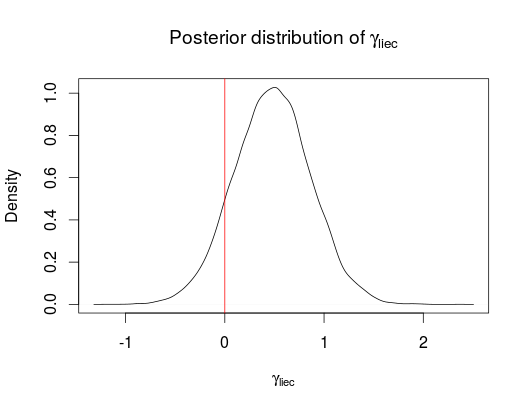
\includegraphics[width=.75\textwidth]{../fig/liec_posterior}
    \label{fig:liec_posterior}
\end{figure}


\subsection{Design}

From the large-n analysis, we find suggestive evidence of an authoritarian legislature having a modest effect on political violence. However, while the matching design alleviates our concern about functional misspecification and incorrect counterfactual, the threat of selection on unobservable remains. Indeed, large variation in the country and country-year intercepts suggests that our model of violence is not yet precise.

Therefore, I follow up the large-n analysis with a survey experiment that aims to affirm a causal prerequisite for my argument. The posited theory about the legislature functioning as an informational and commitment device hinges on the assumption that having legislature actually prompts the co-opted elites to participate in the forum. Otherwise, if the opposition does not consider the legislature to be an effective arena for policy change, then neither can the legislative bargaining provide an attractive alternative to violence nor can the regime gain information about the opposition's capability.

The survey experiment is as follows. Conceptually, the treatment is a country ``having an elected legislature,'' which cannot be randomized. However, in our survey design we can prompt the respondents to think about the legislature as a bargaining arena. My survey question is included in Vietnam's annual business survey PCI (Provincial Competitiveness Index) as follows:\footnote{The PCI is the largest annual business survey in Vietnam, which is designed to assess the ease of doing business, economic governance, and administrative reform efforts \citep{Malesky2013}. This year the surveys reaches 8,013 firms. The PCI is already well-known and implemented regularly, raising no concern that the business may respond differently if they are aware of being studied (i.e. the Hawthorne effect).}

\begin{quote}
(Control prompt) We want to understand how business participate in the process of economic policy making

(Treatment prompt) We want to understand how business participate in the process of economic policy making, \textit{especially since the National Assembly has recently included more delegates that are businessmen} (emphasis added)

Question: Approaching National Assembly delegates to express opinions about economic polices is effective or not?
\end{quote}

Vietnam is an appropriate case for the experiment because Vietnam's growing business sector is being co-opted into the National Assembly. Like China, Vietnam has liberalized its economy while resisting political liberalization. In its 1992 Constitution, drafted when economic reform was already started, the Vietnamese Communist Party (VCP) asserted its role as the vanguard party that commanded the leadership role of the country. At the same time, economic liberalization has created a new class of private entrepreneurs, whose growth becomes increasingly crucial to the country's prosperity and the regime's stability especially when the state-owned sector continues to sluggishly perform \citep{Avery1993}.

Given this mismatch between political and economic power, Vietnam is an insightful case study of the co-optation theory with the new class of capitalists being the potential opposition. Indeed, after the 1992 Constitutional revision, the Vietnamese National Assembly (VNA) has included more diverse and assertive, amending law proposed by the executive, albeit without rejecting it. The representation of businessmen and women in the National Assembly has also increased. In 2007 only 1 out of 30 self-nominated candidates won seat in the VNA, while in 2011 4 out of 15 candidates won seats, including two of the country's best known capitalists \citep{Ruwitch2011}.




\appendix
\section{Appendix A: Bayesian hierarchical model diagnostic}
\label{sec:modeldiagnostic}



\end{document}
